%Correct the file name.
%X: book number
%Y: part number
%ZZZ: page number in three digits. So page 3 would be 003.

\documentclass[11pt]{amsbook}

\usepackage{../HBSuerDemir}	% ------------------------

\begin{document}

% ++++++++++++++++++++++++++++++++++++++
\hPage{b2p1/260}
% ++++++++++++++++++++++++++++++++++++++
% 
 \begin{hEnumerateArabic}
  \setcounter{enumi}{207}
  
  \item
  Find T, N, B, $\kappa$ at he given point of the given curve: \\
     \begin{hEnumerateAlpha}
       \item 
       $r(t) = e^t\cos t i + e^t\sin t j + e^tk, A\hPairingParan{1,0,1}$
       \item
       $r(t) = (1+t)i + (3-t)j + (2t+4)k, B(4,0,10)$
       \item
       $r(t) = 2 Ch\frac{t}{2}i + 2Sh\frac{t}{2}j + 2tk, C(2,0,0)$
     \end{hEnumerateAlpha}
  \item
  Find the equation of the FRENET planes of the curve \\
  $\vec r = \sin 3ti + \cos 3tj + 2t^{\frac{3}{2}}k$ at $(0,1,0)$
  
  \item
  Consider the space curve \\
  $$r: x = \frac{(t-a)^3(t-b)}{t} , y = \frac{(t-a)(t-b)^3}{t} , z = t^3$$
  show that if the osculating plane at a point $P$ passes through $Q$ on $r$, the osculating plane at $Q$ passes through P.
  
  \item
  Prove that
  \begin{hEnumerateAlpha}
       \item 
       $(T^\prime,T^{\prime\prime}, T^{\prime\prime\prime}) = \kappa^3(\kappa \tau^\prime-\kappa^\prime\tau) = \kappa^5 \frac{d}{ds}(\frac{\tau}{\kappa})$
       \item
       $(B^\prime,B^{\prime\prime}, B^{\prime\prime\prime}) = \tau^3(\kappa^\prime\tau - \kappa \tau^\prime) = \tau^5 \frac{d}{ds}(\frac{\kappa}{\tau})$
  \end{hEnumerateAlpha}
  
  \item
  Prove that \\
  $ B = \dot r x \ddot r / K \dot s^3$, $N = (\dot s \ddot r- \ddot s \dot r) / \kappa \dot s^2$, $\kappa^2 = (\ddot r^2 - \dot s^2)/\dot s^4$. and \\
  $ \tau = (\dot r \ddot r \dddot r)/\kappa^2\dot s^6$
  
  \item 
  Prove 
  \begin{hEnumerateAlpha}
       \item 
       $r^\prime \cdot r^{\prime\prime} = 0$ , $r^\prime r^{\prime\prime\prime} = -\kappa^2$ , $r^\prime \cdot r^{\prime\prime\prime} = -3\kappa\kappa^\prime$
       \item
       $r^{\prime\prime\prime} \cdot r^{\prime\prime\prime} = \kappa^\prime \kappa^{\prime \prime} + 2 \kappa^3 \kappa^\prime + \kappa^2\tau\tau^\prime + \kappa\kappa^\prime\tau^2$
       \item
       $T^\prime \cdot B^\prime = -K\tau$
  \end{hEnumerateAlpha}
  
  \item
  Squaring $r^{\prime\prime\prime} = -\kappa^2\tau + \kappa^\prime N + K\tau B$ obtain 
  \begin{hEnumerateAlpha}
    \item
    $\tau^3 = \frac{1}{\kappa^2} r^{\prime \prime \prime2} - \kappa^2 - (\frac{\kappa^\prime}{\kappa})^2$
    \item
    $r^{\prime\prime\prime} = -3\kappa\kappa^\prime T +(\kappa^{\prime\prime} - \kappa^3 - KT^2)N + (2K^\prime T + KT^\prime)B$
  \end{hEnumerateAlpha}
  
  \item
  Given $r^{(n)} = a_nT + b_nN + c_nB$ show that

 \end{hEnumerateArabic}
% 



% =======================================================
\end{document}  

%==== templates ====

%==== environments ====

%\begin{figure}[htb]
%	\centering
%	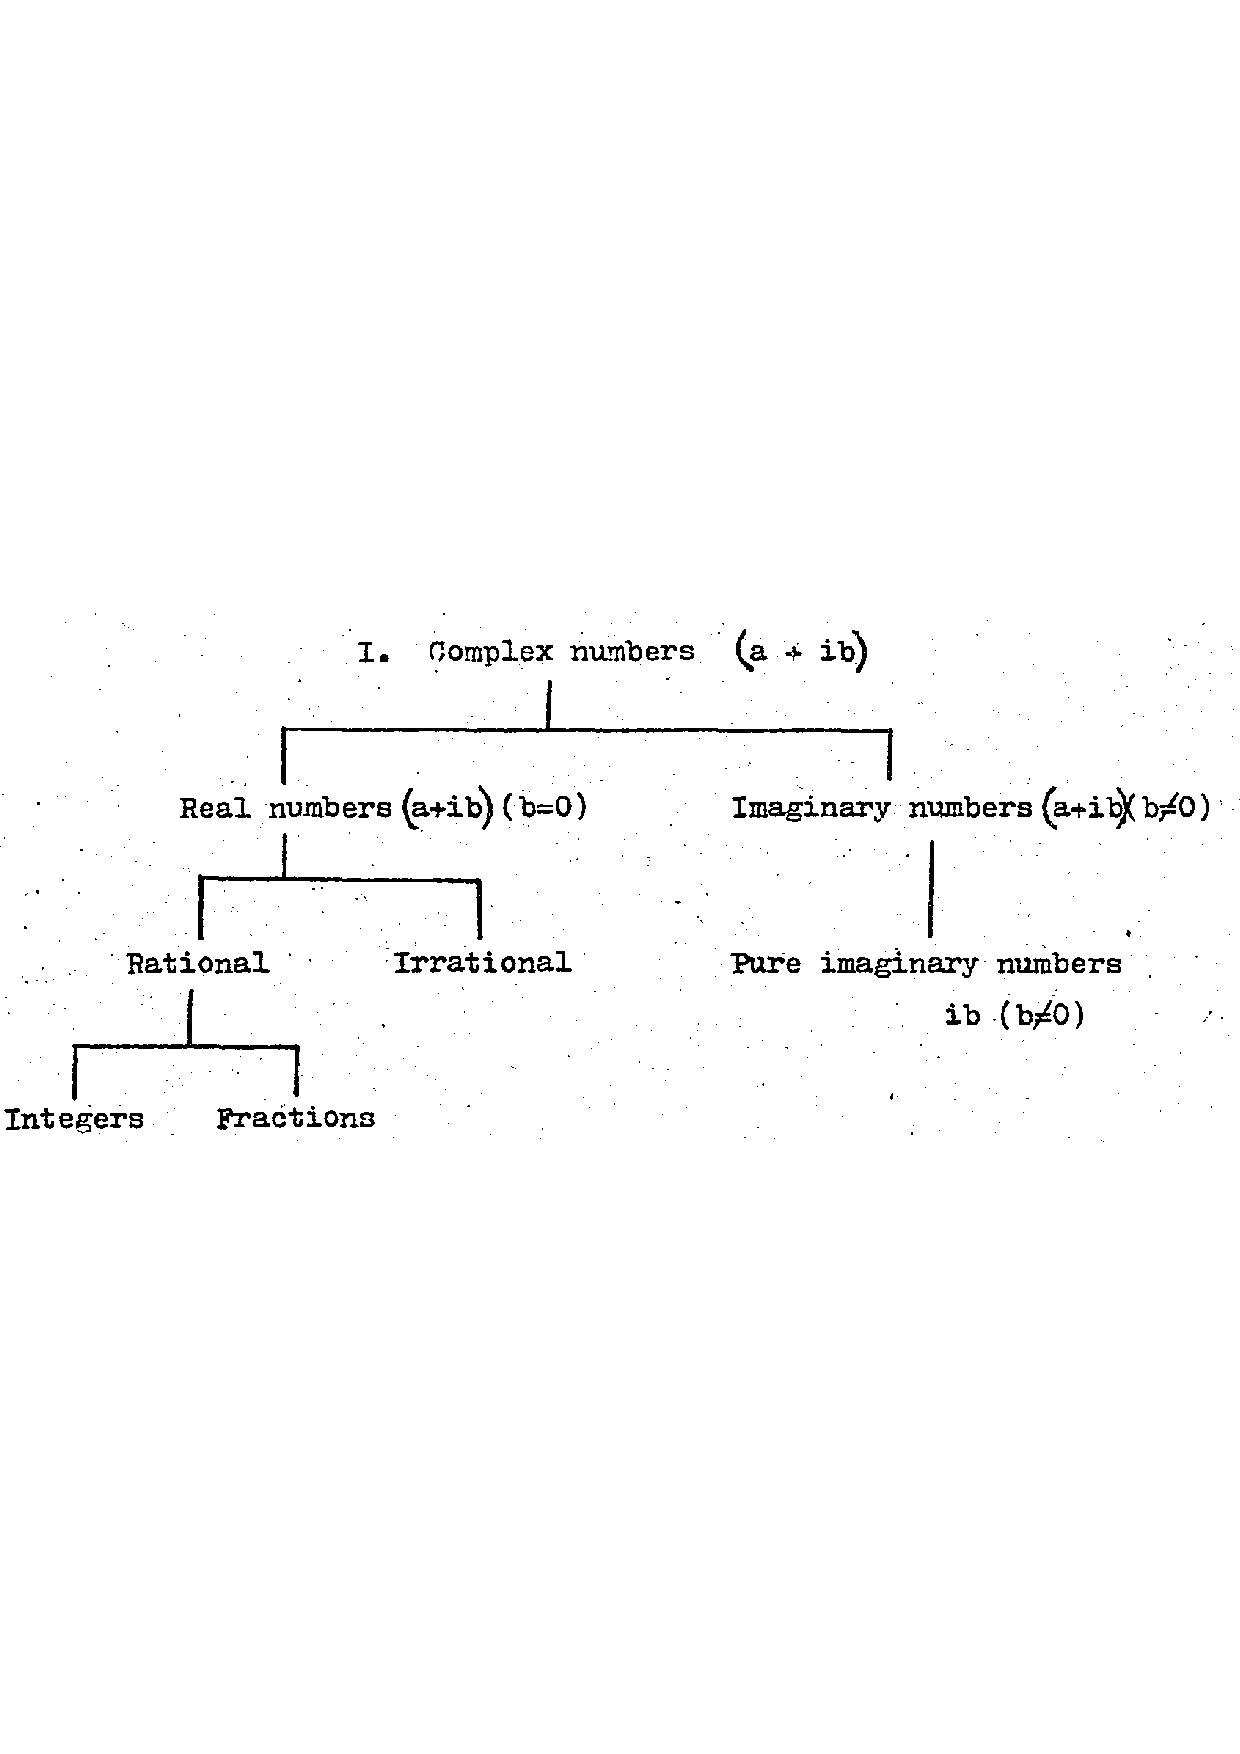
\includegraphics[width=0.9\textwidth]{images/SD-1-1p15A}
%	\caption{Classification of complex numbers}
%	\label{fig:classificationOfComplexNumbersA}
%\end{figure}

%\begin{center}
%\begin{tabular}{cc}
%\end{tabular}
%\end{center}

%\begin{exmp}
%\begin{hSolution}
%\end{hSolution}
%\end{exmp}

%\begin{hEnumerateAlpha}
%\end{hEnumerateAlpha}

%\begin{hEnumerateRoman}
%\end{hEnumerateRoman}

%$
%\begin{bmatrix}
%\end{bmatrix}
%$

%\frac{aaaa}{bbb}
%\frac{a_{n}}{b_{n}}
%\left( aaaa \right)
%\Longrightarrow

%\begin{multicols}{2}
%	bb
%\columnbreak
%	aa
%\end{multicols}
